\documentclass[10pt,a4paper]{article}
\usepackage[utf8]{inputenc}
\usepackage{amsmath}
\usepackage{amsfonts}
\usepackage{amssymb}
\usepackage{graphicx}
\usepackage{epstopdf}
\usepackage[ngerman]{babel}
\usepackage[ngerman]{translator}
\usepackage{listings}
\usepackage[colorlinks=true,
        linkcolor=black,
        citecolor=black,
        filecolor=black,
        pagecolor=black,
        urlcolor=black,
        bookmarks=true,
        bookmarksopen=true,
        bookmarksopenlevel=3,
        plainpages=false,
        pdfpagelabels=true]{hyperref}

%Paket laden
\usepackage[
	nonumberlist, %keine Seitenzahlen anzeigen
	acronym,      %ein Abkürzungsverzeichnis erstellen
	toc,          %Einträge im Inhaltsverzeichnis
	section]      %im Inhaltsverzeichnis auf section-Ebene erscheinen
	{glossaries}

%Befehle für Glossar
\makeglossaries
\newglossaryentry{Feld}{
	name=Feld,
	description={Ein Feld ist eine quadratische Fläche mit einem Steitenmaß von mindestens 10cm. Es stellt die kleinste Einheit eines
	Spielfeldes dar}
}

\parindent 0pt
\pagestyle{headings}

\let\oldsection\section
\renewcommand{\section}{\newpage \oldsection}

\title{
	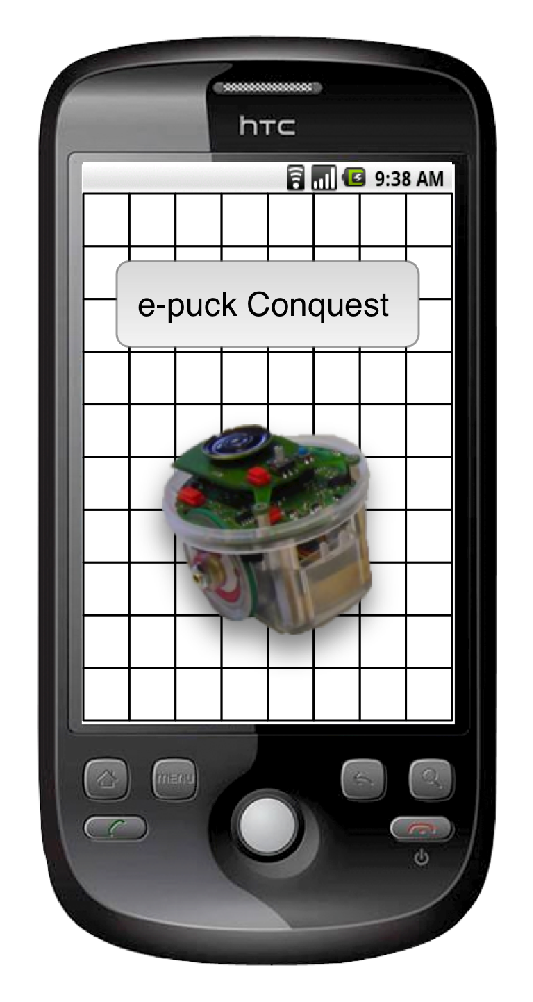
\includegraphics[height=10cm]{logo.eps} \\
	\vspace{1cm}
	Entwurf
}
\author{SEP - ITS - Team \\ Max Binder, Florian Bürchner, Martin Freund, \\Florian Lorenz,
											Andreas Poxrucker, Andreas Wilhelm}
\begin{document}
	\maketitle
	\newpage
	\tableofcontents	
	\newpage

	\section{Einleitung}
		Dieses Dokument stellt den konzeptionellen Entwurf des e-puck Conquest Systems dar. Dabei handelt es sich um ein
		verteiltes System mit bis zu sechs e-puck Roboter und einem Android-Smartphone. \\ \\
		Die Roboter sollen ein Spielfeld möglichst zeiteffizient in Kooperation mit den anderen Teilnehmern erkunden.
		Auf dem Smartphone werden die gesammelten Kartendaten dargestellt. Außerdem kann ein e-puck zur manuellen Steuerung
		ausgewählt werden. \\ \\
		Die Kommunikation der Roboter wird über ein Bluetooth-Netzwerk in Ringarchitektur abgewickelt. (siehe Abbildung 1). Trotz
		der Beschränkung des Bluetooth-Moduls auf sieben direkte Verbindungen wird durch diese Architektur eine hohe Skalierbarkeit
		gewährleistet. \\
		Das Smartphone verbindet sich zu einem ausgewählten e-puck, Nachrichten werden mittels Broadcast über das Netzwerk an alle 
		anderen Teilnehmer versendet.
		
		Dieses Dokument stellt den konzeptionellen Entwurf des e-puck Conquest Systems dar. Hierbei handelt es sich um ein
		verteiltes System mit bis zu sechs  e-puck Roboter und einem Android-Smartphone. \\
		Die Roboter haben die Aufgabe ein Spielfeld möglichst zeiteffizient in Kooperation mit den anderen Teilnehmern zu erkunden.
		Auf dem Smartphone werden die gesammelten Kartendaten dargestellt, außerdem kann ein e-puck zur manuellen Steuerung
		ausgewählt werden. \\
		Die Kommunikation der Roboter wird über ein Bluetooth-Netzwerk in einer Ringarchitektur behandelt (siehe Abbildung 1). Trotz
		der Beschränkung des Bluetooth-Moduls auf 7 direkte Verbindungen wird durch diese Architektur eine hohe Skalierbarkeit
		gewährleistet. Das Smartphone verbindet sich zu einem ausgewählten e-puck, Nachrichten werden über Broadcast über
		das Netzwerk an alle anderen Teilnehmer versendet.

		\begin{figure}[h]
			\centering
			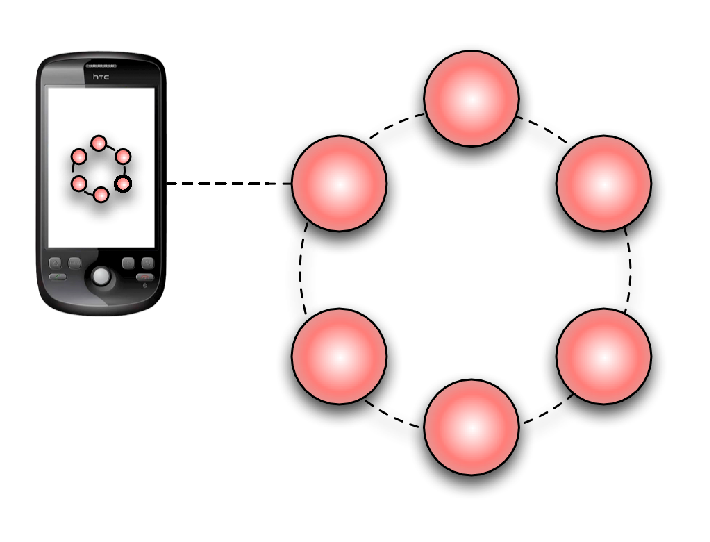
\includegraphics[width=10cm]{images/system.eps}
  			\caption{Verteiltes e-puck System}
  		\end{figure}
  		
		Der Entwurf des Systems wird zur besseren Übersicht in die Bereiche \textit{e-puck Roboter}, \textit{Smartphone} und
		\textit{Kommunikation} aufgeteilt. \\
		Das Ziel ist ein möglichst hohes Maß an	Qualität, Wartbarkeit und Erweiterbarkeit. Dazu ist ein sinnvolles Systemdesign unter
		Verwendung mehrerer verschiedener Entwurfsmuster und Architekturen in allen Bereichen erforderlich. \\ \\
		Weiterhin werden in den folgenden Abschnitten die verwendeten Datentypen und Schnittstellen der Komponenten erläutert. Die beschränkten
		Ressourcen der Roboter erzwingen hierbei einen möglichst effizienten Aufbau. Insbesondere stellt der interne
		Arbeitsspeicher sowie die Rechenleistung der e-pucks eine Einschränkung für den Entwurf dar.
				
	\section{e-Puck Roboter}
  				
		\subsection{Architektur}
		Die Software des e-puck wird als Schichtenarchitektur mit wachsendem Abstraktionsgrad entworfen. \\
		Jede Schicht besteht aus einer oder mehreren Komponenten. Diese sind teilweise wiederum aus mehreren
		Schichten aufgebaut. \\
		
		\begin{figure}[h]
			\centering
			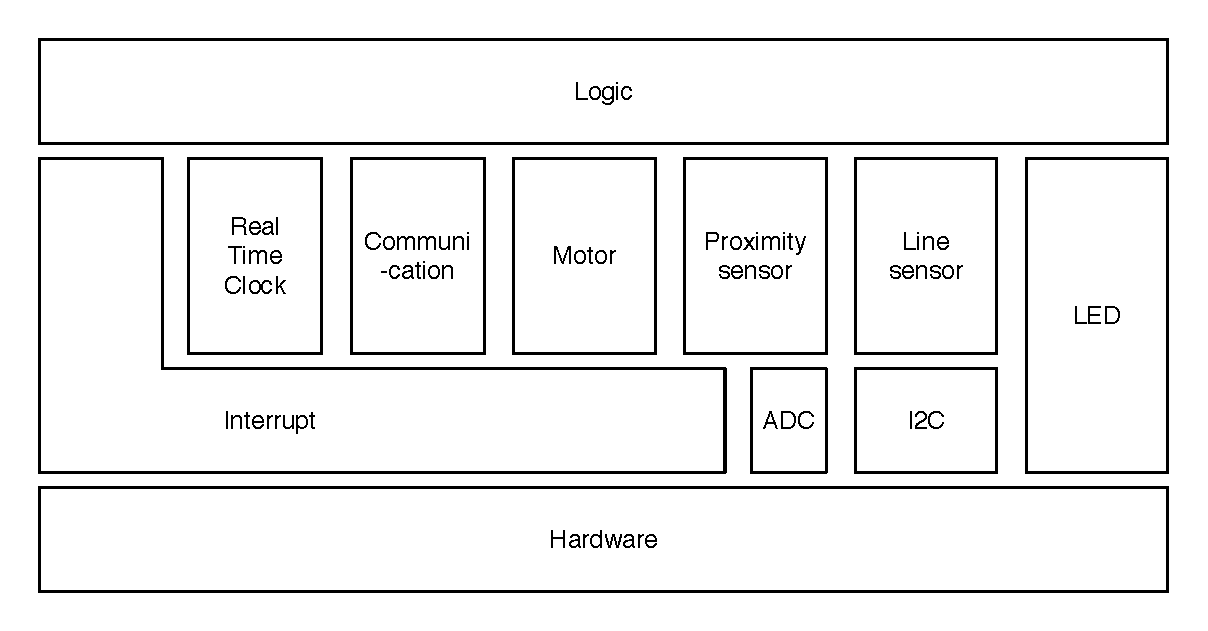
\includegraphics[width=10cm]{images/e-puck_architecture.eps}
  			\caption{Architektur der Software des e-puck}
  		\end{figure}
		
		Die folgenden Abschnitte beschreiben die einzelnen Komponenten der Architektur näher.
		 
			\paragraph*{Komponente `Interrupt'}
			Die Komponente `Interrupt' bietet einfache Funktionen zum globalen Ein- und Ausschalten von Interrupts und zur Festlegung
			von Interrupt-Prioritäten. Außerdem können gesetzte Interrupt-Flags gelöscht werden. \\ \\
			Diese Funktionen werden in den Komponenten `Timer', `Motor', `Communication' und `IR proximity sensor' sowie
			in der darüber liegenden Logikschicht verwendet. \\
			
			Externe Datenstrukturen: keine \\
			
			Strukturelle Gliederung der Komponente:
			\begin{verbatim}  
			hal_int.h, hal_int.c, hal_int_types.h
			\end{verbatim}

			\paragraph*{Komponente `Real-Time-Clock'}
			Die `Real-Time-Clock'-Komponente stellt eine Echtzeituhr bereit. Diese speichert die aktuelle Laufzeit des e-puck Roboter und löst in
			regelmäßigen Abständen Interrupts aus.
			Außerdem können Callbacks für zeitgesteuerte Funktionen anderer Komponenten registriert werden. \\
			
			Strukturelle Gliederung:
			\begin{verbatim}  
			hal_rtc.h, hal_rtc.c, hal_rtc_types.h
			\end{verbatim}
			
			Externe Datenstrukturen: keine
			
			\paragraph*{Komponente `Communication'}
			Die Komponente `Communication' stellt einfache Funktionen zum Aufbau und Verwaltung der Ringstruktur des Bluetooth-Netzwerks bereit.
			Sie enthält außerdem Funktionen zum Senden und Empfangen von Bluetooth-Nachrichten.\\
			 
			Die Modul besteht aus zwei aufeinander aufbauenden Komponenten mit wachsendem Abstraktionsgrad:
			
				\subparagraph*{hal\_uart1}
				Diese Komponente bildet die hardwarenahste Schicht des Kommunikationsmoduls. \\
				Sie enthält Funktionen zur Initialisierung des UART. Insbesondere werden das Datenformat und die Datenrate festgelegt.
				Darüber hinaus können die Sende- und Empfangs-Interrupts des UART konfiguriert werden. Die zu den Interrupts gehörigen Interrupt
				Service Routinen sind ebenfalls Teil der Komponente. \\
				Auch die Kontrolle des Transmitter (Tx)- und Receiver (Rx)-Ringpuffers wird in diesem Modul realisiert. \\
				Das Senden und Empfangen von Nachrichten erfolgt asynchron. \\
				
				Strukturelle Gliederung:
				\begin{verbatim}  
				hal_uart.h, hal_uart.c, hal_uart1_types.h
				\end{verbatim}
				
				Externe Datenstrukturen: \\
				ringbuf\_SContext\_t: Zustand des Ringpuffers
				
				\lstset{language = C, tabsize = 4}
				\begin{lstlisting}[frame = single]
typedef struct {
	uint8_t* lpui8Storage;
	uint16_t ui16Size;
	volatile uint16_t ui16ReadIndex;
	volatile uint16_t ui16WriteOffset;
} ringbuf_SContext_t;
				\end{lstlisting}
				
				\subparagraph*{com}
				`com' enthält Funktionen zur Generierung von Raw-Messages (Nachrichten, die vom Bluetooth-Modul versendet werden
				können) und zur Aufbereitung von eingehenden Raw-Nachrichten aus der darunter liegenden `hal\_uart'-Schicht. \\
				
				Strukturelle Gliederung:
				\begin{verbatim}  
				btm.h, btm.c, btm_types.h
				\end{verbatim}
				
				Externe Datenstrukturen: \\
				com\_SMessage\_t: Format der Raw-Nachrichten
				
				\lstset{language = C, tabsize = 4}
				\begin{lstlisting}[frame = single]
typedef struct {
	uint16_t ui16type;
	uint8_t aui8Data[30];
} com_SMessage_t;
				\end{lstlisting}
				
			\paragraph*{Komponente `Motor'}
			Das Modul `Motor' stellt Funktionen zur Verfügung, die die Voraussetzung für die High-Level-Steuerung der Bewegung des e-puck bilden.
			Die Komponente initialisiert und kontrolliert die Timer für die Steuerung der beiden Schrittmotoren und gewährleistet deren korrekte
			Ansteuerung. \\
			Außerdem werden Funktionen bereit gestellt, mit denen die Geschwindigkeit der beiden Motoren eingestellt werden kann und deren
			Schrittzähler gelesen und gesetzt werden können. \\
			
			Strukturelle Gliederung:
				\begin{verbatim}  
				hal_motor.h, hal_motor.c, hal_motor_types.h
				\end{verbatim}
						
			\paragraph*{Komponente `ADC'}
			Die Komponente `ADC' kapselt Funktionen zur Initialisierung der Analog-Digital-Wandler und zum einfachen Auslesen der Register
			mit den konvertierten Werten. \\
			Das Funktionen der Komponente bilden eine wichtige Grundlage für die Verwendung der IR-Abstandssensoren und werden vom Modul `IR 
			proximity sensor' verwendet.
			
			Strukturelle Gliederung:
				\begin{verbatim}  
				hal_adc.h, hal_adc.c, hal_adc_types.h
				\end{verbatim}
			
			\paragraph*{Komponente `I2C'}
			Die Komponente `I2C' initialisiert die Datenrate und die Masterfunktionalität des I2C-Moduls.
			Außerdem werden grundlegenden Übertragungsfunktionen wie Adressierung, Lesen und Schreiben zur Verfügung gestellt. \\
			
			Strukturelle Gliederung:
				\begin{verbatim}  
				hal_i2c.h, hal_i2c.c
				\end{verbatim}
			
			\paragraph*{Komponente `IR proximity sensor'}
			Es erfüllt im wesentlichen zwei Hauptaufgaben.
			Zunächst findet eine Initialisierung statt. Hierbei wird das Abtastintervall mit dem die Sensoren ausgelesen werden definiert und der 
			Timer eingerichtet, mit dem das Abtastintervall betrieben wird.
			Weiterhin stellt dieses Modul die Funktionen zum Auslesen der IR-Sensoren zur Verfügung. Dabei werden Funktionen der `ADC'-Komponente 		
			verwendet. \\
			
			Strukturelle Gliederung:
				\begin{verbatim}  
				sen_prox.h, sen_prox.c, sen_prox_types.h
				\end{verbatim}
			
			\paragraph*{Komponente `Line sensor'}
			Die Hauptaufgabe dieser logischen Komponente liegt darin, die Daten der IR-Abstandssensoren aus dem I2C-Bus auszulesen um sie später 
			einem Regler zur Verfügung zu stellen, der gewährleistet, dass der jeweilige Roboter seine Linie nicht verlässt. \\
			
			Strukturelle Gliederung:
				\begin{verbatim}  
				sen_line.h, sen_line.c, sen_line_types.h
				\end{verbatim}
			
			\paragraph*{Komponente `LED'}
			Zunächst werden sämtliche für die LEDs benötigten Hardware-Register initialiserit. Sobald dies geschehen ist, kann durch diese Komponente 
			die Ansteuerung der LEDs am e-puck übernommen werden.
			
			Strukturelle Gliederung:
				\begin{verbatim}  
				hal_led.h, hal_led.c
				\end{verbatim}
				
				
		\begin{figure}[h]
			\centering
			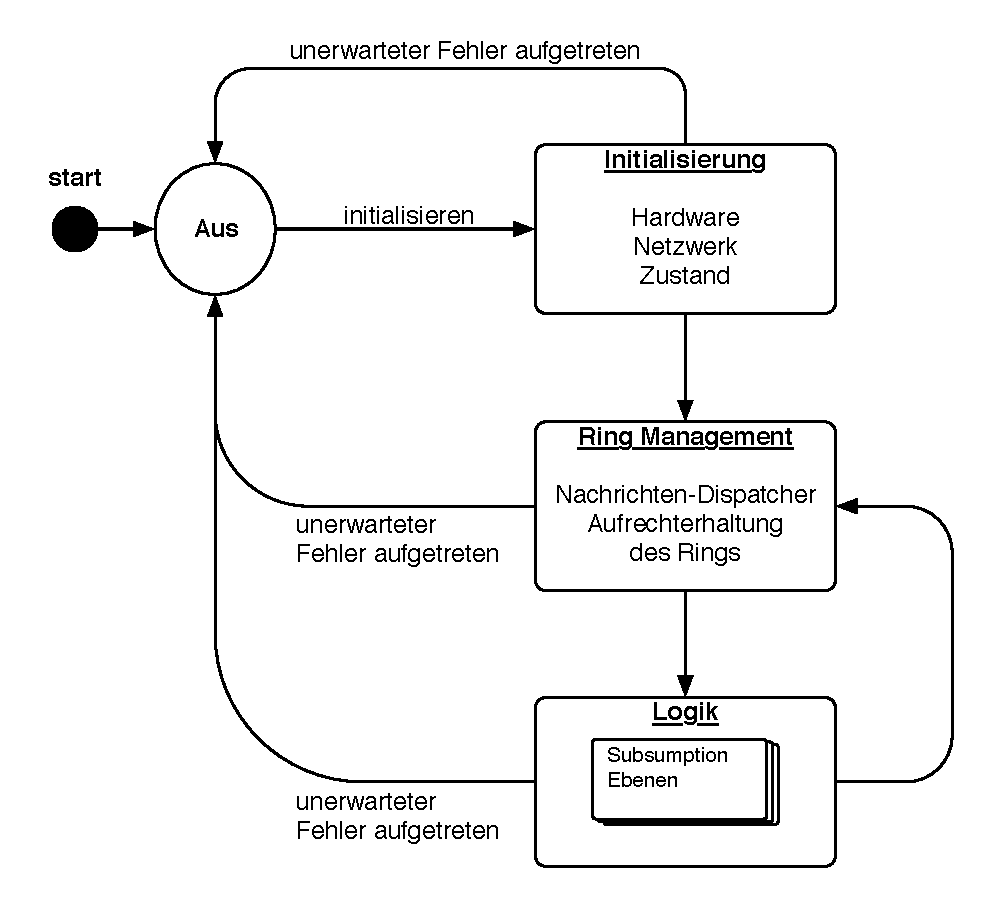
\includegraphics[width=9cm]{images/e-puck.eps}
  			\caption{Ablaufmodell}
  		\end{figure}
			
		\section{Smartphone}
		\subsection{Model-View-Controller (MVC) Architektur}
			Die Daten- bzw. Benutzer-Interaktion der Android-Anwendung wird mit einer MVC-Architektur aufgebaut. Dies ermöglicht ein
			flexibles Programmdesign, das eine Wiederverwendbarkeit von Komponenten sowie eine reduzierte Komplexität gewährleistet.
			Die Daten, wie z.B. Karteninformationen oder Roboterpositionen, können dadurch von den zugehörigen Darstellungen getrennt werden
			(\textit{Separation of Concerns}). Es werden hierbei drei Dialoge (\textit{Activities}) verwendet, je ein Dialog für Kartenansicht, Steuerung und
			Statistik. Bei diesem Entwurf hat die View-Schicht keinen direkten Zugriff auf das Model, dieser wird vollständg vom
			Controller übernommen. Gemäß den Entwicklerrichtlinien für Android-Anwendungen 
			\footnote{Android - User Interface (\url{http://developer.android.com/guide/topics/ui/index.html})} gehören die Activity-Klassen der
			View logisch zum	Controller. Die Model-Schicht (Proxies) erhält über die Bluetooth-Schnittstelle Aktualisierungen der e-puck Roboter,
			welche den Zustand ändern.\\
			Die beschriebenen Steuerungs- und Dialogabläufe werden hier nur rudimentär zum Verständnis erwähnt. Eine genauere Erläuterung ist in
			Kapitel [TODO] zu finden
			\begin{figure}[h]
			\centering
			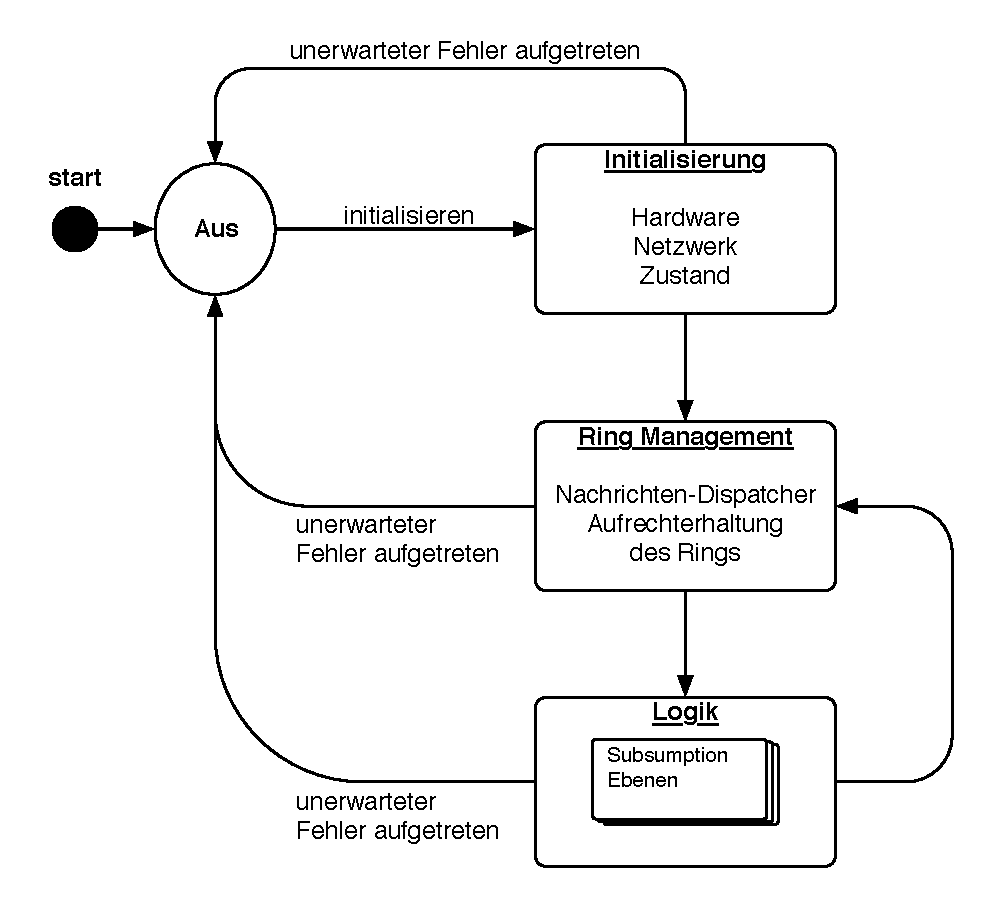
\includegraphics[width=10cm]{images/e-puck.eps}
  			\caption{Ablaufdiagramm}
  			\end{figure}
  			
	\section{Smartphone}
			\begin{figure}
				\centering
				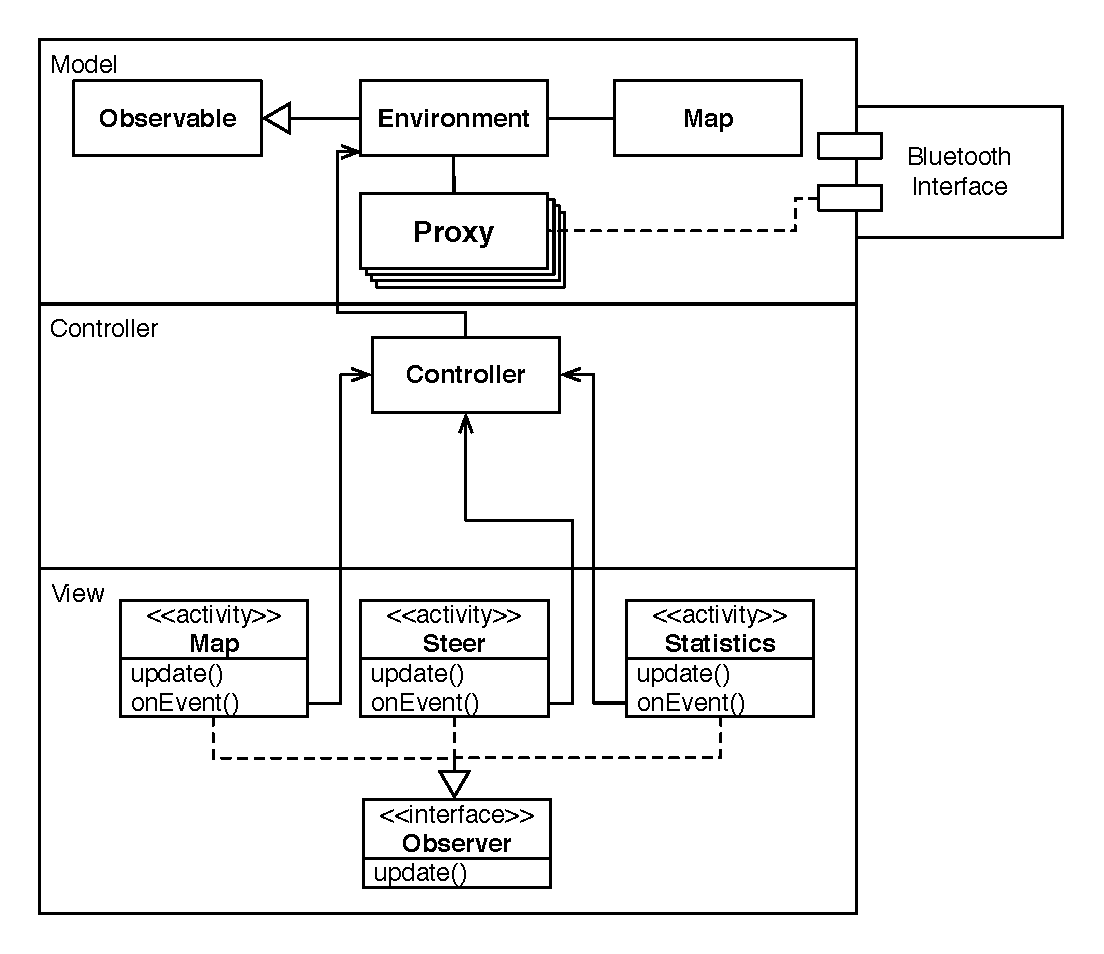
\includegraphics[width=10cm]{images/android_mvc.eps}
  				\caption{Model-View Controller Architektur}
  			\end{figure}	
			\paragraph*{Model}
  				Die Model-Schicht der Architektur speichert als zentrale Komponente sämtliche Daten bzgl. Karten- und e-puck-Informationen. 
  				Sie beinhaltet außerdem die Applikationslogik der Android-Anwendung. Die Kommunikation nach außen findet über das
  				angeschlossene Bluetooth-Interface statt. Die Klasse \textit{Environment} erbt von der Klasse \textit{Observable} und verarbeitet
  				die Aktualisierungen der Roboter. Die Klasse wird als Singleton realisiert, da hier globale Zustandsdaten und Karteninformation
  				für die Anzeige gespeichert werden. Informationen der einzelnen Roboter, sowie deren Ablaufsteuerung, werden in den Instanzen
  				der Klasse \textit{Proxy} verwaltet (siehe Kapitel [TODO]). Diese Insanzen werden in einer Attributsliste der Klasse \textit{Environment}
  				gehalten und besitzen auch selbst einen Verweis auf diese Klasse. Bei	Zustandsänderung der \textit{Proxy}-Instanzen bzw. bei
  				Änderung der Kartendaten werden die registrierten Views benachrichtigt.
  			\paragraph*{View}
  				Die Präsentationskomponenten der MVC-Architektur sind für die Ausgabe der Model-Daten zuständig und bilden eine
  				Abstraktionsschicht zwischen der Präsentation der Anwendung, dem Model und dem Benutzer. Die Schicht besteht aus den drei
  				Klassen	\textit{Map}, \textit{Steer} und \textit{Statistics}. \textit{Map} ist für die Kartendarstellung
  				verantwortlich, \textit{Steer} stellt die Steuerungsbedienelemente dar und \textit{Statistics} beinhaltet statistische
  				Informationen.  Damit die View-Klassen als \textit{Activities} für die Android-Applikation verwendet werden können, müssen sie
  				das Interface \textit{Activity} implementieren. Für die Verwendung als View der MVC-Architektur muss zusätzlich das Interface
  				\textit{Observer} implementiert werden. Jede einzelne View registriert sich bei der Klasse \textit{Environment} als Observer,
  				um bei Zustandsänderungen vom Model benachrichtigt zu werden. Benutzereingaben auf den Dialogen werden über
  				die Ereignisbehandler-Methoden des \textit{Activity}-Interface an das Model weitergegeben. Somit gehören diese Handler-Methoden
  				im Sinne der MVC-Architektur der Controller-Schicht an.
  			\paragraph*{Controller}
  				Der Controller nimmt Eingaben aus den verschiedenen View Klassen entgegen und leitet diese bereinigt und normalisiert an die
  				Model-Schicht weiter. Hier wird also eine Abstraktionsschicht eingeführt, welche die Verbindung zwischen Benutzer-Interaktionen
  				und dem Model beschreibt. Zur Controller-Schicht gehört neben den Ereignisbehandler-Methoden der View Klassen die Klasse
  				\textit{Controller}, welche für die zentrale Steuerung der Model Schicht verantwortlich ist.
  		\subsection{Nachrichtenbehandlung}
  			Wir verwenden das Chain-of-Responsibility-Pattern in unserem Projekt, um Nachrichten, die von den e-puck Robotern an das Handy
  			geschickt werden zu analysieren und weiter zu verarbeiten. Die Grundidee hinter diesem Pattern ist, dass die Nachricht durch eine Liste
  			von konkreten Handlerklassen, die von einer abstrakten Handlerklasse erben, gereicht wird und der richtige Handler die Nachricht
  			verarbeitet. Sobald eine Nachricht von einem Handler erkannt und bearbeitet wurde gibt er true zurück. Falls sich der Handler nicht
  			verantwortlich für die Nachricht fühlt gibt er sie an den nächsten Handler weiter. Falls auch der letzte Handler mit der Nachricht nicht
  			umzugehen weiß, gibt er den Rückgabewert false zurück.Im Gegensatz zu herkömmlichen Nachrichtenbearbeitungen wird hier ein
  			hohes Maß an Flexibilität erreicht und es das Hinzufügen eines neuen Nachrichtentyps wird erleichtert, da nur eine neue Klasse in die
  			Liste der Handler hinzugefügt werden muss. \\ \\
  			Vorteile:
  			\begin{itemize}
  				\item Der Absender braucht sich nicht zu kümmern, wer genau die Nachricht verarbeitet (implizieter Empfänger)
  				\item Unabhängigkeit zwischen Sender und Empfänger (Entkopplung)
  				\item Sehr gut erweiterbar, falls ein neuer Nachrichtentyp hinzugefügt werden soll
  				\item Mehrere Klassen kümmern sich um die Verarbeitung, d.h. die Fehlersuche und -behandlung wird vereinfacht
  				\item Größere Flexibilität bei der Bearbeitung von Nachrichten
  				\item Mithilfe des Rückgabewerts wird erkannt, ob eine Nachricht behandelt wurde
  			\end{itemize}  
  			Teilnehmer:
   			\begin{itemize}
  				\item Handler\\Definiert ein Interface für die Requests\\Besitzt Zeiger auf nächstes Listenelement
  				\item Konkrete Handler\\Größere Flexibilität bei der Bearbeitung von Nachrichten\\
  					Mithilfe des Rückgabewerts wird erkannt, ob eine Nachricht behandelt wurde
  				\item Client \\ Ruft Funktion handlerequest(Nachricht) auf ersten Listenelement der Handler auf
  			\end{itemize}   	
			\begin{figure}[h]
				\centering
				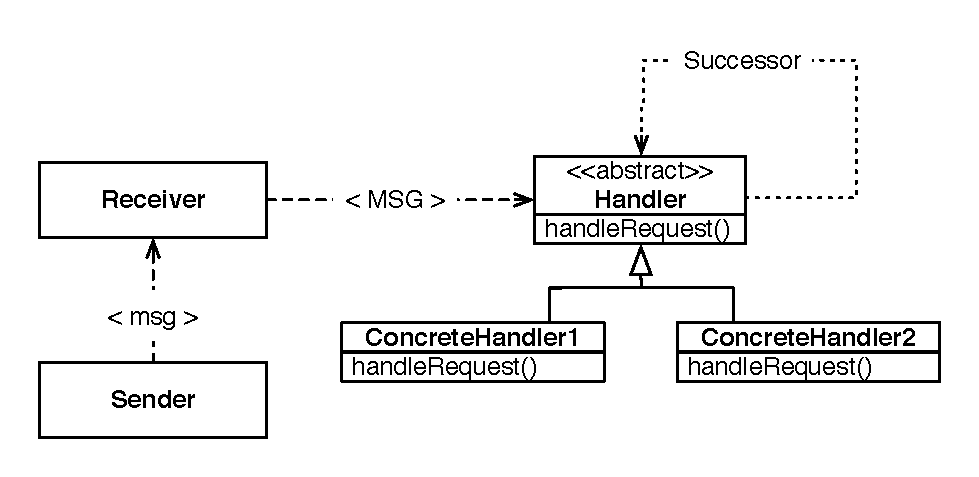
\includegraphics[width=10cm]{images/android_handler.eps}
  				\caption{Chain of Responsibility - Entwurfsmuster}
  			\end{figure}	
  			Erklärung der Abbildung:
   			\begin{enumerate}
  				\item Die Bluetoothschnittstelle leitet eine einkommende Nachricht weiter an eine Client-Klasse, die eine Liste aus konkreten Handlern,
  					die von der abstrakten Klasse Handler erben, enthält.
  				\item Diese Klasse gibt die Nachricht an den ersten Handler seiner Liste weiter und ruft dort die Funktion handlerequest(Nachricht),
  					die den Rückgabetyp Boolean hat, auf.
  				\item Der Handler leitet die Nachricht an seinen direkten Nachfolger weiter und ruft dort wieder handlerequest(Nachricht) auf, sofern
  					er nicht für die Bearbeitung der Nachricht zuständig ist. In diesem Fall behandelt er die Nachricht entsprechend und gibt true zurück
  				\item Der Handler, der keinen Nachfolger mehr hat gibt den Wert false zurück und somit weiß der Client dass für die Nachricht kein
  					entsprechender Handler zur Verfügung steht.  					
  			\end{enumerate}   
  		\subsection{Repräsentation der e-puck Roboter}
  			Der Zugriff auf einzelne e-pucks aus der Android Applikation heraus erfolgt durch Einsatz des Proxy Patterns. Dieses dient als Schnittstelle
  			zwischen der Programmlogik und dem Bluetooth Interface. Die Proxy Klasse wird als abstrakte Oberklasse implementiert,wobei jede Instanz
  			dieser Klasse, genau einen e-puck repräsentiert. Diese Stellvertreterobjekte speichern die Zustände der zugehörigen Roboter und beinhalten
  			alle Funktionen um Daten des Roboters abzurufen oder zu setzen.
			\begin{figure}[h]
				\centering
				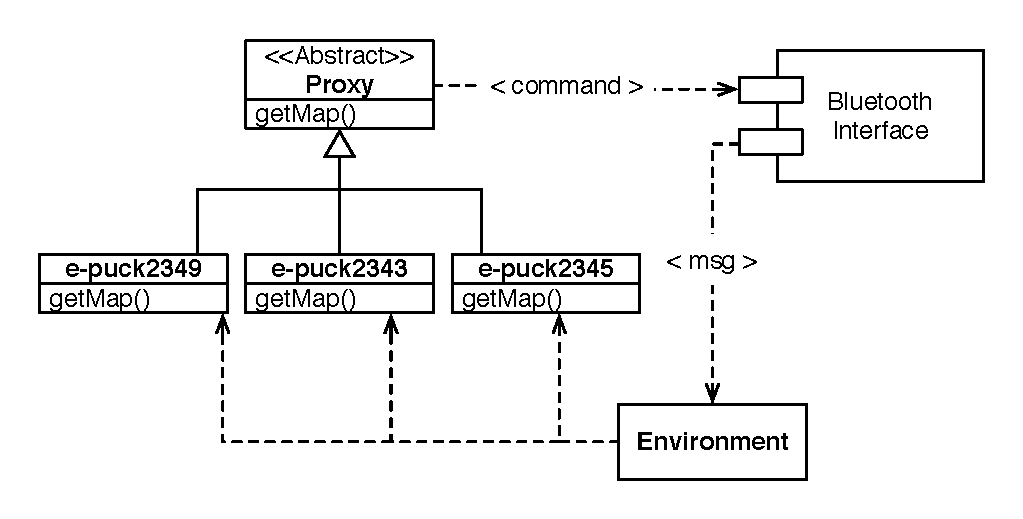
\includegraphics[width=10cm]{images/android_proxy.eps}
  				\caption{Proxy - Entwurfsmuster}
  			\end{figure}	
  			Durch das Einsparen von Logik im Bluetooth Interface und Auslagern in die Proxy Klasse ist die Austauschbarkeit der Robotermodelle gegeben
  			und man bleibt flexibel für die Einführung neuer Befehle. \\ \\
  			Beim Entdecken eines neuen, noch unbekannten e-pucks durch das Bluetooth Interface wird für diesen eine neue Instanz der Proxy Klasse
  			angelegt. Die Kommunikation mit diesem Roboter ist ausschließlich über dieses Objekt möglich.\\ \\
  			Das Erkunden von neuen Knoten wird vom e-puck zunächst an das Bluetooth Interface weitergegeben und die Informationen anschließend
  			in der Environment Klasse verarbeitet. Die Zustände der einzelnen Roboter, wie zum Beispiel die aktuelle Position, wird aber an die
  			entsprechenden Proxy Instanzen vermittelt und gespeichert.\\ \\
  			Der andere Weg führt von der Benutzereingabe über das Environment, welches je nach Befehl die richtige Funktion am Objekt des zugehörigen
  			e-pucks aufruft. Von dort werden Befehle über das Bluetooth Interface an den Roboter gesendet.
  		\subsection{Erzeugung der Views}
  			Ein Ziel der Anwendungs-Architektur ist die Möglichkeit, den Austausch von View-Elementen in einfacher Weise zu ermöglichen. Für diesen
  			Zweck wird das Abstract-Factory Entwurfsmuster zur Erzeugung einer Gruppe von Steuerelementen verwendet. Die Art sowie das Aussehen der
  			Benutzeroberfläche ist damit von der Logik getrennt und neue Darstellungen können einfach hinzugefügt werden.
			\begin{figure}[h]
				\centering
				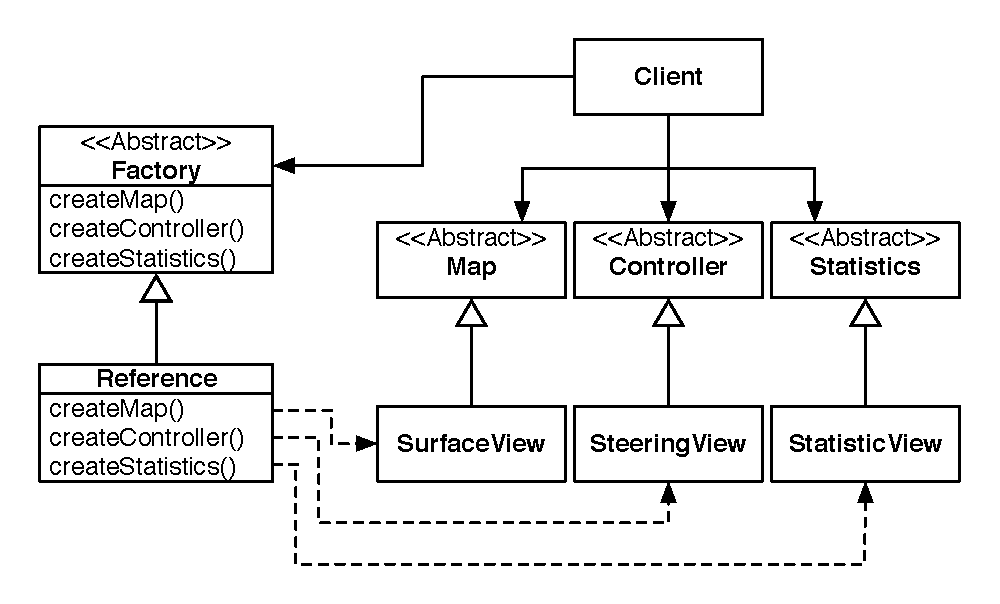
\includegraphics[width=10cm]{images/android_abstrfact.eps}
  				\caption{Abstract Factory - Entwurfsmuster}
  			\end{figure}
  			Die Klasse \textit{Factory} dient als Muster zur Erzeugung ganzer ``Familien'' von Views. Um im Fall der Android-Anwendung die konkreten
  			Dialoge für Karte, Steuerung und Statistik zu erstellen, existiert die Klasse \textit{Reference}, welche von \textit{Factory} erbt. Diese sorgt
  			wiederum dafür, dass die konkreten Acitvity-Klassen \textit{SurfaceView}, \textit{SteeringView} und \textit{StatisticsView} der Android
  			-Applikation korrekt erzeugt werden. Um die Repräsentation der Dialoge für den Benutzer einfach austauschbar zu gestalten, erben diese Klassen
  			von entsprechenden abstrakten Oberklassen. Der Client hat somit lediglich die Aufgabe, eine Instanz einer konkreten Factory-Klasse zu
  			erzeugen, der restliche Ablauf kann für jede beliebige Familie von Dialogen gleich erfolgen. \\ \\
  			Die Verwendung des Abstract Factory - Entwurfsmusters hat hier den Vorteil, dass konkrete Dialog-Klassen isoliert behandelt werden können.
  			Außerdem macht es den Austausch ganzer Familien einfach und fördert Konsistenz über gesamte Dialog-Familien. Der entscheidende Punkt für
  			den sinnvollen Einsatz, liegt bei dem Entwurf der abstrakten Activity-Klassen \textit{Map}, \textit{Controller} und \textit{Statistics}. Zum Einen
  			wird die Erweiterung der entsprechenden Schnittstellen aufwändig, sobald mehrere konkrete Ableitungen existieren. Zusätzlich müssen im
 			Vorhinein sämtliche benötigten Methoden in diese Klassen aufgenommen werden, um die vollständige Funktionalität gewährleisten zu können. 
	\section{Kommunikation}
				
			
	\newpage	
	%Glossar ausgeben
	\printglossary[style=altlist,title=Glossar]
						
\end{document}